
\section{ʵ������}
\label{sec3_3}

\subsection{ʵ�鳡��������}
Many experiments were carried out using different parameters for the validation of the approach to segment the aorta from CTA.
In our case, the CTA series in DICOM format had been converted to the form of XML first.
Then the converted data was fed into the feature image production branch and input level sets generation branch.
The resulting data from the two branches were sent to geodesic active contours module in order to generate the final results.
Finally, the marching cubes method is used to visualize the segmented data.
The experiments were all run on a machine with Intel's 2.83GHz Core 2 Quad CPU and 4GB RAM.

The input series was obtained by a 128-slice Siemens SOMATOM Definition Flash CT with the slice thickness of 0.6mm.
And the series contains the patient's entire abdominal aorta.
For illustrative purposes, a typical slice was selected from the series.
To reduce the computation time, the region that contains the major branches of the abdominal vasculature in the selected image were cropped (see Fig. \ref{fig_roi}).
\begin{figure}[t]
\centering
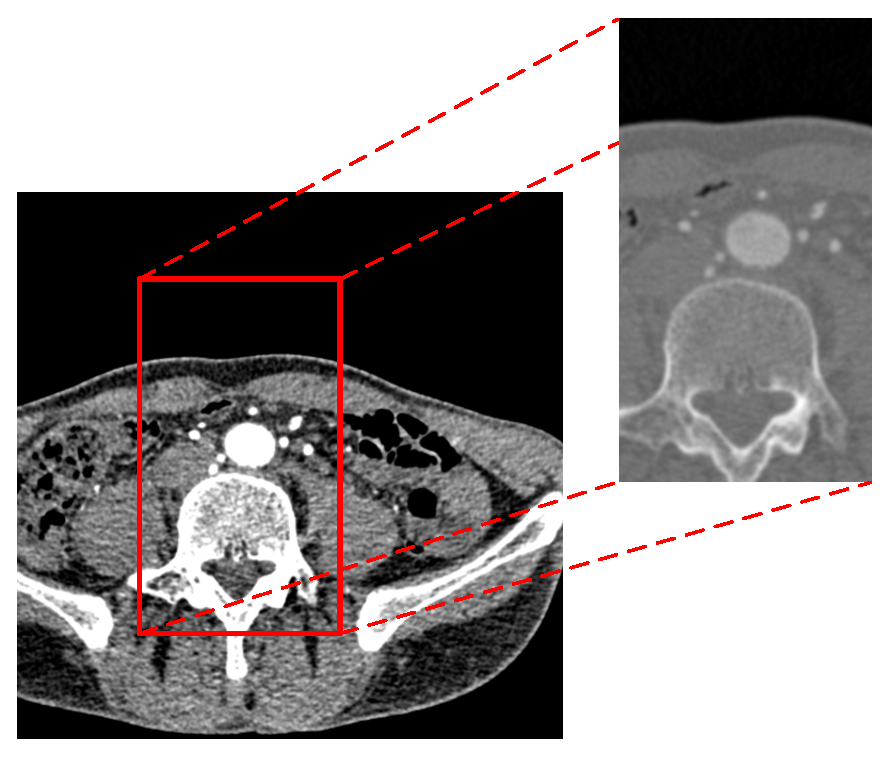
\includegraphics[width=2.5in]{figures/chap03/ROI.eps}
\caption{A typical ROI extraction of the original slice.}
\label{fig_roi}
\end{figure}
% Then the segmentation process was split into two branches first and then merged into the main evolution pipeline.
%This two-branching structure is built due to the two essential requirements of geodesic active contours module: the feature images and initial level sets.

\subsection{����ͼ��ļ���}
In the feature image production branch, the following preprocessing tasks were performed sequentially:
\begin{enumerate}
\item removing noises without affecting the edges;
\item computing the gradient magnitude pixel-wisely;
\item mapping the intensity into the required feature.
\end{enumerate}
At the beginning, a level-set curvature method with variable conductance was utilized to perform the smoothing task.
It is an edge-preserving smoothing method that can remove the unnecessary noises from the images while preserving the nature of the boundaries of the objects.
The image was smoothed nicely and the boundaries of the aorta even the minor vessels (which means weaker edges) were preserved (see Fig. \ref{fig:Smoothing}).
Then the gradient magnitude module was introduced to fulfill the requirements of gradient computing.
It computes the magnitude of the gradient pixel-wisely for the image by performing the convolution with the first order derivatives of a Gaussian kernel defined by (\ref{eqn:Gaussian}).
%The only parameter of the kernel is its deviation $\sigma$ and we set it to 0.9.
The edges of the vessels, bones, and skins were extracted completely in the resulting image (see Fig. \ref{fig:Gradient}).
After computing the magnitude of the gradient, the non-linear intensity mapping was employed to generate the edge potential map.
The choices of the parameters in (\ref{eqn:Sigmoid}) heavily depends on extreme values of the pixel intensities in the gradient image.
In this case, to reverse the relationship between objects (in low intensities in the gradient map) and their edges (in high intensities in the gradient map), $m$ was set to be a negative value and $n$ to be a positive value which is larger than $|m|$.
The mapping produced the expected feature image with the proximities of the edges of the objects in zero intensity (see Fig. \ref{fig:Sigmoid}).
This made the evolution of the level sets driven by (\ref{eqn:Geodesic3}) propagated faster in the ``flat area" (with uniformly high intensities), whilst much slower (in a speed of about zero) in the ``ridge" (with rapid decreasing intensities).
\begin{figure*}[t]
\centering
%\subfloat[Smoothing with edge preserving (Conductance parameter = 0.9)]{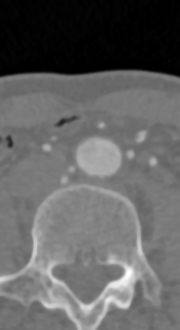
\includegraphics[width=1.2in]{fig/dcm_smoothing.jpg}%
\subfloat[]{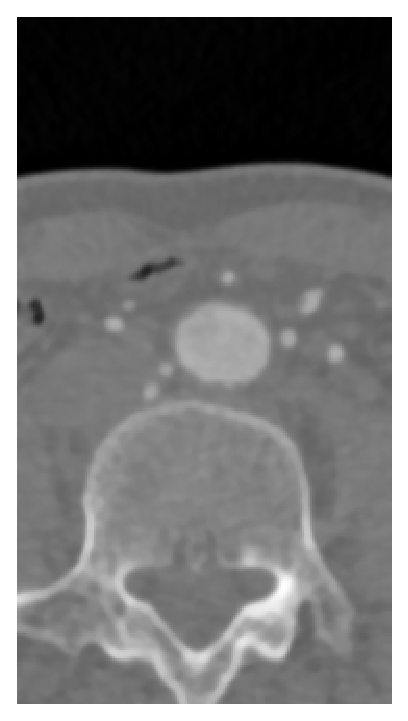
\includegraphics[width=1.2in]{figures/chap03/dcm_smoothing.eps}%
\label{fig:Smoothing}}
\hfil
%\subfloat[Computation of magnitude of gradient with Gaussian kernel ($\sigma = 0.9$)]{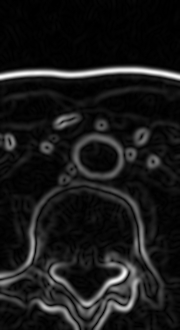
\includegraphics[width=1.2in]{fig/dcm_gradient.jpg}%
\subfloat[]{
\includegraphics[width=1.2in]{figures/chap03/dcm_gradient.eps}%
\label{fig:Gradient}}
\hfil
%\subfloat[Nonlinear mapping using an S-shaped function ($m = -3$, $n = 20$)]{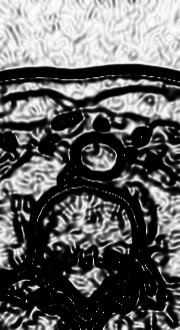
\includegraphics[width=1.2in]{fig/dcm_sigmoid.jpg}%
\subfloat[]{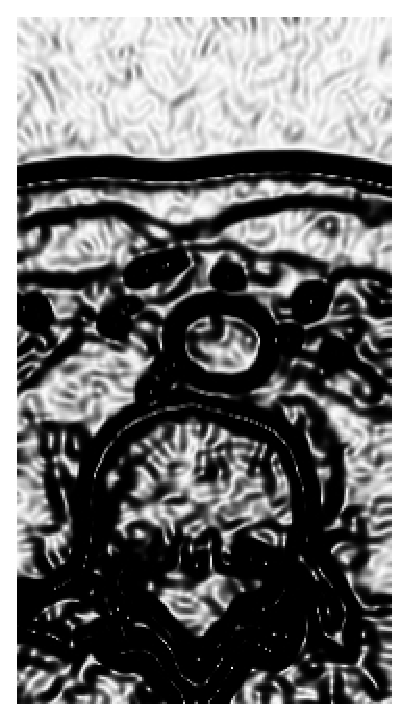
\includegraphics[width=1.2in]{figures/chap03/dcm_sigmoid.eps}%
\label{fig:Sigmoid}}
\caption{Producing the feature image in three steps: (a) smoothing with edge preserving ($\text{conductance parameter} = 9.0$); (b) computation of magnitude of gradient with Gaussian kernel ($\sigma = 0.9$); (c) nonlinear mapping using an S-shaped function ($m = -3$, $n = 20$).}
%\caption{Producing the feature image.}
\label{fig:PotentialImageGeneration}
\end{figure*}
\begin{figure*}[t]
\centering
%\subfloat[Thresholding]{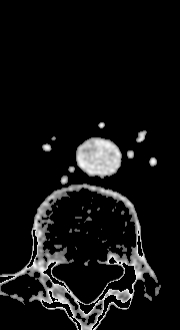
\includegraphics[width=1.2in]{fig/dcm_threshold.jpg}%
\subfloat[]{
\includegraphics[width=1.2in]{figures/chap03/dcm_threshold.eps}%
\label{fig:Threholding}}
\hfil
%\subfloat[Level set evolution using fast marching method]{
\includegraphics[width=1.2in]{fig/dcm_fastMarching.jpg}%
\subfloat[]{
\includegraphics[width=1.2in]{figures/chap03/dcm_fastMarching.eps}%
\label{fig:FastMarching}}
\hfil
%\subfloat[Edge detection using geodesic active contours]{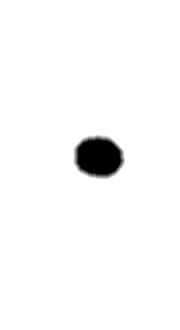
\includegraphics[width=1.2in]{fig/dcm_geodesic.jpg}%
\subfloat[]{
\includegraphics[width=1.2in]{figures/chap03/dcm_geodesic.eps}%
\label{fig:GeodesicActiveContours}}
\hfil
%\subfloat[Binary thresholding]{
\includegraphics[width=1.2in]{fig/dcm_out.jpg}%
\subfloat[]{
\includegraphics[width=1.2in]{figures/chap03/dcm_out.eps}%
\label{fig:BinaryThresholding}}
\caption{Level set evolution: (a) thresholding ($\text{lower threshold} = 300\text{HU}$, $\text{higher threshold} = 2000\text{HU}$); (b) initial level set evolution from one seeding point using fast marching method; (c) edge detection using geodesic active contours; (d) binary thresholding to inverse the pixel intensities (intensity of the light area: $255$, intensity of the dark area: $0$).}
\label{fig:LevelSetEvolution}
\end{figure*}

\subsection{ˮƽ���ݽ�}
The initial level set generation branch works for the level sets that required by the geodesic active contours module.
In this process, the thresholding module was called first to trim off the irrelevant organs with lower intensities, such as lungs, liver, kidneys, bowels, stomach, etc. (see Fig. \ref{fig:Threholding}).
%In our case, we set the lower and upper threshold values at 300HU (HU is short for Hounsfield Unit) and 2000HU, respectively.
This can further reduce the hunger for memory and dramatically shorten the computation time.
When finished this, the fast marching module is provoked to generate the initial interfaces.
One seed located interior of the region representing the aorta was fed to this module in this two dimensional image.
% And these seeds evolved the interfaces surrounding themselves respectively towards each other (see Fig. \ref{fig:FastMarching}).
And the time of arrival $T(x,y)$ given in (\ref{eqn:Curves}) were computed (see Fig. \ref{fig:FastMarching}).
Considering the prolonged geometric nature of the aorta and the characteristics of the algorithm, multiple seeding points inside the space representing the aorta should be fed in the three dimension case to acquire better results and much shorter computation time.
% We set the stopping time for the fast marching filter in order to shorten the time for the generation of initial level sets.

% \subsection{Geodesic Evolution}
The geodesic active contours evolution began working when all the preceding computation finished.
The module took the feature image and the initial contours as its inputs.
The contours evolved by the drive defined by (\ref{eqn:Geodesic3}) with the feature image as their reference.
The segmentation module evolved the contours until the edges were met (see Fig. \ref{fig:GeodesicActiveContours}).
After that, a binary thresholding step was performed to fill the inner area of the final contours as the light zone while the outer area as the dark zone.
This result is illustrated in Fig. \ref{fig:BinaryThresholding}.
All the parameters chosen manually to make the drive suitable to evolve the contour to the expected results were reused in the three dimensional case.

\subsection{���ڷָ����ı����ؽ�}
Finally, the resulting volume were processed using the marching cubes method \cite{Lorensen1987MC}.
The isovalue corresponding to the edge of the lumen of abdominal aorta was picked manually.
Here the higher threshold value of the binary thresholder was provided as the isovalue for the isosurface extraction.
This ensured that the rendered surface representing the surfaces of the lumen of the aorta.
The final visualization model is depicted in Fig. \ref{fig:VisualizationModel}.
%From this figure, we can see that the lumen of the aorta was extracted successfully using the approach described here.
\begin{figure}[t]
\centering
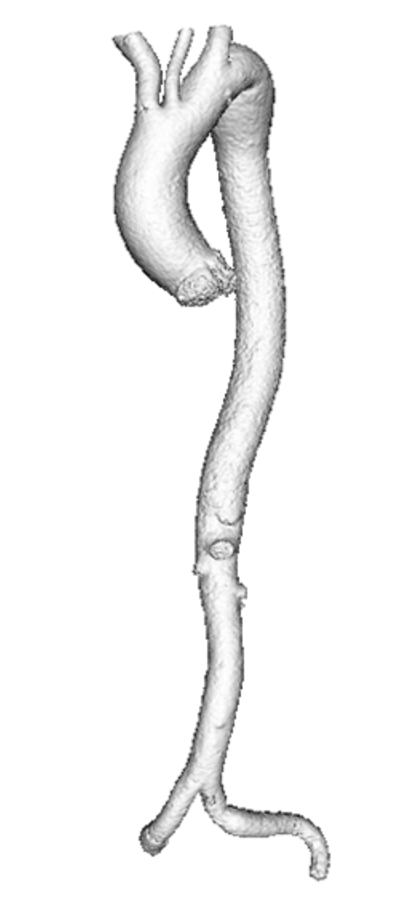
\includegraphics[width=1.1in]{figures/chap03/model.eps}
\caption{3-D surface model of the lumen of the aorta.}
\label{fig:VisualizationModel}
\end{figure} 